\section{Poglavlje}

Ovako citiram Pytorch \cite{pytorch} i Numpy \cite{numpy}. Ovako citiram vise stvari \cite{backpropagation_1986,neuronska_mreza_1943, perceptron_1958}. Lorem ipsum dolor sit amet, consectetur adipiscing elit, sed do eiusmod tempor incididunt ut labore et dolore magna aliqua. Ut enim ad minim veniam, quis nostrud exercitation ullamco laboris nisi ut aliquip ex ea commodo consequat.

%ht! -> ako zelim da mi slika bude vise manje na istom mjestu gdje sam je stavio u source code-u
%width=\textwidth -> sirina slike jednaka stranici, ovisno o slici moze se koristit i scale=0.6 itd.
\begin{figure}[ht!]
    \centering
    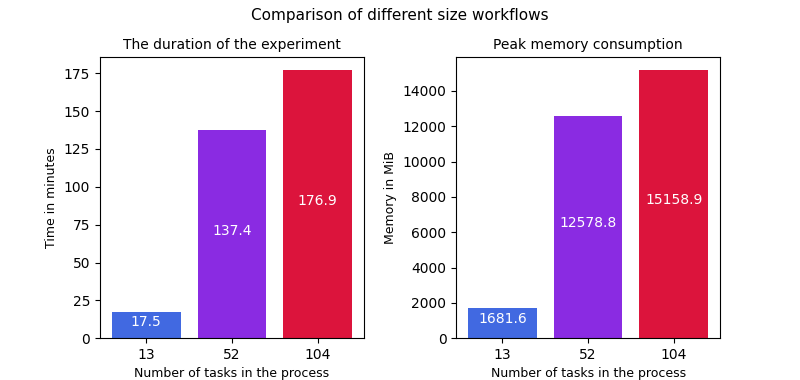
\includegraphics[width=\textwidth]{slike/test-slika.png}
    \caption{Ovo je naslov slike}
    \label{fig:slika}
\end{figure}

Ovako referenciram sliku \ref{fig:slika}. Ut enim ad minim veniam, quis nostrud exercitation ullamco laboris nisi ut aliquip ex ea commodo consequat. Duis aute irure dolor in reprehenderit in voluptate velit esse cillum dolore eu fugiat nulla pariatur.

\subsection{Podpoglavlje}

Lorem ipsum dolor sit amet, consectetur adipiscing elit, sed do eiusmod tempor incididunt ut labore et dolore magna aliqua. Ut enim ad minim veniam, quis nostrud exercitation ullamco laboris nisi ut aliquip ex ea commodo consequat. Duis aute irure dolor in reprehenderit in voluptate velit esse cillum dolore eu fugiat nulla pariatur.

%Tablice su malo problematicne u latex-u, preporucam https://www.tablesgenerator.com/

\begin{table}[ht!]
\centering
\begin{tabular}{@{}cccc@{}}
\toprule
 Test      & Varijabla 2 & Varijabla 3 & Varijabla 4 \\ \midrule
Test 1 & 2.12341     & 3.12341234  & 4.1235      \\
Test 2 & 5.123       & 6.34        & 7.123       \\ \bottomrule
\end{tabular}
\caption{Ovo je naslov tablice}
\label{tab:my-table}
\end{table}

Ovako referenciram tablicu \ref{tab:my-table}. Ut enim ad minim veniam, quis nostrud exercitation ullamco laboris nisi ut aliquip ex ea commodo consequat. Duis aute irure dolor in reprehenderit in voluptate velit esse cillum dolore eu fugiat nulla pariatur.

\subsubsection{PodPodPoglavlje}\label{pod-pod-poglavlje}

Lorem ipsum dolor sit amet, consectetur adipiscing elit, sed do eiusmod tempor incididunt ut labore et dolore magna aliqua. Ut enim ad minim veniam, quis nostrud exercitation ullamco laboris nisi ut aliquip ex ea commodo consequat. Duis aute irure dolor in reprehenderit in voluptate velit esse cillum dolore eu fugiat nulla pariatur. Excepteur sint occaecat cupidatat non proident, sunt in culpa qui officia deserunt mollit anim id est laborum. Lorem ipsum dolor sit amet, consectetur adipiscing elit, sed do eiusmod tempor incididunt ut labore et dolore magna aliqua. Ut enim ad minim veniam, quis nostrud exercitation ullamco laboris nisi ut aliquip ex ea commodo consequat. Duis aute irure dolor in reprehenderit in voluptate velit esse cillum dolore eu fugiat nulla pariatur. 

\subsection{Drugo podpoglavlje}

Ovako mogu referencirat poglavlje \ref{pod-pod-poglavlje} u radu. I ako mi treba fusnota\footnote{Ovo je fusnota...}. Excepteur sint occaecat cupidatat non proident, sunt in culpa qui officia deserunt mollit anim id est laborum. Lorem ipsum dolor sit amet, consectetur adipiscing elit, sed do eiusmod tempor incididunt ut labore et dolore magna aliqua. Ut enim ad minim veniam, quis nostrud exercitation ullamco laboris nisi ut aliquip ex ea commodo consequat. Duis aute irure dolor in reprehenderit in voluptate velit esse cillum dolore eu fugiat nulla pariatur. Excepteur sint occaecat cupidatat non proident, sunt in culpa qui officia deserunt mollit anim id est laborum. Lorem ipsum dolor sit amet, consectetur adipiscing elit, sed do eiusmod tempor incididunt ut labore et dolore magna aliqua. Ut enim ad minim veniam, quis nostrud exercitation ullamco laboris nisi ut aliquip ex ea commodo consequat. Duis aute irure dolor in reprehenderit in voluptate velit esse cillum dolore eu fugiat nulla pariatur. Excepteur sint occaecat cupidatat non proident, sunt in culpa qui officia deserunt mollit anim id est laborum. Lorem ipsum dolor sit amet, consectetur adipiscing elit, sed do eiusmod tempor incididunt ut labore et dolore magna aliqua. Ut enim ad minim veniam, quis nostrud exercitation ullamco laboris nisi ut aliquip ex ea commodo consequat. Duis aute irure dolor in reprehenderit in voluptate velit esse cillum dolore eu fugiat nulla pariatur.
